% Options for packages loaded elsewhere
\PassOptionsToPackage{unicode}{hyperref}
\PassOptionsToPackage{hyphens}{url}
\PassOptionsToPackage{dvipsnames,svgnames,x11names}{xcolor}
%
\documentclass[
  letterpaper,
  DIV=11,
  numbers=noendperiod]{scrartcl}

\usepackage{amsmath,amssymb}
\usepackage{lmodern}
\usepackage{iftex}
\ifPDFTeX
  \usepackage[T1]{fontenc}
  \usepackage[utf8]{inputenc}
  \usepackage{textcomp} % provide euro and other symbols
\else % if luatex or xetex
  \usepackage{unicode-math}
  \defaultfontfeatures{Scale=MatchLowercase}
  \defaultfontfeatures[\rmfamily]{Ligatures=TeX,Scale=1}
\fi
% Use upquote if available, for straight quotes in verbatim environments
\IfFileExists{upquote.sty}{\usepackage{upquote}}{}
\IfFileExists{microtype.sty}{% use microtype if available
  \usepackage[]{microtype}
  \UseMicrotypeSet[protrusion]{basicmath} % disable protrusion for tt fonts
}{}
\makeatletter
\@ifundefined{KOMAClassName}{% if non-KOMA class
  \IfFileExists{parskip.sty}{%
    \usepackage{parskip}
  }{% else
    \setlength{\parindent}{0pt}
    \setlength{\parskip}{6pt plus 2pt minus 1pt}}
}{% if KOMA class
  \KOMAoptions{parskip=half}}
\makeatother
\usepackage{xcolor}
\setlength{\emergencystretch}{3em} % prevent overfull lines
\setcounter{secnumdepth}{-\maxdimen} % remove section numbering
% Make \paragraph and \subparagraph free-standing
\ifx\paragraph\undefined\else
  \let\oldparagraph\paragraph
  \renewcommand{\paragraph}[1]{\oldparagraph{#1}\mbox{}}
\fi
\ifx\subparagraph\undefined\else
  \let\oldsubparagraph\subparagraph
  \renewcommand{\subparagraph}[1]{\oldsubparagraph{#1}\mbox{}}
\fi

\usepackage{color}
\usepackage{fancyvrb}
\newcommand{\VerbBar}{|}
\newcommand{\VERB}{\Verb[commandchars=\\\{\}]}
\DefineVerbatimEnvironment{Highlighting}{Verbatim}{commandchars=\\\{\}}
% Add ',fontsize=\small' for more characters per line
\usepackage{framed}
\definecolor{shadecolor}{RGB}{241,243,245}
\newenvironment{Shaded}{\begin{snugshade}}{\end{snugshade}}
\newcommand{\AlertTok}[1]{\textcolor[rgb]{0.68,0.00,0.00}{#1}}
\newcommand{\AnnotationTok}[1]{\textcolor[rgb]{0.37,0.37,0.37}{#1}}
\newcommand{\AttributeTok}[1]{\textcolor[rgb]{0.40,0.45,0.13}{#1}}
\newcommand{\BaseNTok}[1]{\textcolor[rgb]{0.68,0.00,0.00}{#1}}
\newcommand{\BuiltInTok}[1]{\textcolor[rgb]{0.00,0.23,0.31}{#1}}
\newcommand{\CharTok}[1]{\textcolor[rgb]{0.13,0.47,0.30}{#1}}
\newcommand{\CommentTok}[1]{\textcolor[rgb]{0.37,0.37,0.37}{#1}}
\newcommand{\CommentVarTok}[1]{\textcolor[rgb]{0.37,0.37,0.37}{\textit{#1}}}
\newcommand{\ConstantTok}[1]{\textcolor[rgb]{0.56,0.35,0.01}{#1}}
\newcommand{\ControlFlowTok}[1]{\textcolor[rgb]{0.00,0.23,0.31}{#1}}
\newcommand{\DataTypeTok}[1]{\textcolor[rgb]{0.68,0.00,0.00}{#1}}
\newcommand{\DecValTok}[1]{\textcolor[rgb]{0.68,0.00,0.00}{#1}}
\newcommand{\DocumentationTok}[1]{\textcolor[rgb]{0.37,0.37,0.37}{\textit{#1}}}
\newcommand{\ErrorTok}[1]{\textcolor[rgb]{0.68,0.00,0.00}{#1}}
\newcommand{\ExtensionTok}[1]{\textcolor[rgb]{0.00,0.23,0.31}{#1}}
\newcommand{\FloatTok}[1]{\textcolor[rgb]{0.68,0.00,0.00}{#1}}
\newcommand{\FunctionTok}[1]{\textcolor[rgb]{0.28,0.35,0.67}{#1}}
\newcommand{\ImportTok}[1]{\textcolor[rgb]{0.00,0.46,0.62}{#1}}
\newcommand{\InformationTok}[1]{\textcolor[rgb]{0.37,0.37,0.37}{#1}}
\newcommand{\KeywordTok}[1]{\textcolor[rgb]{0.00,0.23,0.31}{#1}}
\newcommand{\NormalTok}[1]{\textcolor[rgb]{0.00,0.23,0.31}{#1}}
\newcommand{\OperatorTok}[1]{\textcolor[rgb]{0.37,0.37,0.37}{#1}}
\newcommand{\OtherTok}[1]{\textcolor[rgb]{0.00,0.23,0.31}{#1}}
\newcommand{\PreprocessorTok}[1]{\textcolor[rgb]{0.68,0.00,0.00}{#1}}
\newcommand{\RegionMarkerTok}[1]{\textcolor[rgb]{0.00,0.23,0.31}{#1}}
\newcommand{\SpecialCharTok}[1]{\textcolor[rgb]{0.37,0.37,0.37}{#1}}
\newcommand{\SpecialStringTok}[1]{\textcolor[rgb]{0.13,0.47,0.30}{#1}}
\newcommand{\StringTok}[1]{\textcolor[rgb]{0.13,0.47,0.30}{#1}}
\newcommand{\VariableTok}[1]{\textcolor[rgb]{0.07,0.07,0.07}{#1}}
\newcommand{\VerbatimStringTok}[1]{\textcolor[rgb]{0.13,0.47,0.30}{#1}}
\newcommand{\WarningTok}[1]{\textcolor[rgb]{0.37,0.37,0.37}{\textit{#1}}}

\providecommand{\tightlist}{%
  \setlength{\itemsep}{0pt}\setlength{\parskip}{0pt}}\usepackage{longtable,booktabs,array}
\usepackage{calc} % for calculating minipage widths
% Correct order of tables after \paragraph or \subparagraph
\usepackage{etoolbox}
\makeatletter
\patchcmd\longtable{\par}{\if@noskipsec\mbox{}\fi\par}{}{}
\makeatother
% Allow footnotes in longtable head/foot
\IfFileExists{footnotehyper.sty}{\usepackage{footnotehyper}}{\usepackage{footnote}}
\makesavenoteenv{longtable}
\usepackage{graphicx}
\makeatletter
\def\maxwidth{\ifdim\Gin@nat@width>\linewidth\linewidth\else\Gin@nat@width\fi}
\def\maxheight{\ifdim\Gin@nat@height>\textheight\textheight\else\Gin@nat@height\fi}
\makeatother
% Scale images if necessary, so that they will not overflow the page
% margins by default, and it is still possible to overwrite the defaults
% using explicit options in \includegraphics[width, height, ...]{}
\setkeys{Gin}{width=\maxwidth,height=\maxheight,keepaspectratio}
% Set default figure placement to htbp
\makeatletter
\def\fps@figure{htbp}
\makeatother

\KOMAoption{captions}{tableheading}
\makeatletter
\makeatother
\makeatletter
\makeatother
\makeatletter
\@ifpackageloaded{caption}{}{\usepackage{caption}}
\AtBeginDocument{%
\ifdefined\contentsname
  \renewcommand*\contentsname{Table of contents}
\else
  \newcommand\contentsname{Table of contents}
\fi
\ifdefined\listfigurename
  \renewcommand*\listfigurename{List of Figures}
\else
  \newcommand\listfigurename{List of Figures}
\fi
\ifdefined\listtablename
  \renewcommand*\listtablename{List of Tables}
\else
  \newcommand\listtablename{List of Tables}
\fi
\ifdefined\figurename
  \renewcommand*\figurename{Figure}
\else
  \newcommand\figurename{Figure}
\fi
\ifdefined\tablename
  \renewcommand*\tablename{Table}
\else
  \newcommand\tablename{Table}
\fi
}
\@ifpackageloaded{float}{}{\usepackage{float}}
\floatstyle{ruled}
\@ifundefined{c@chapter}{\newfloat{codelisting}{h}{lop}}{\newfloat{codelisting}{h}{lop}[chapter]}
\floatname{codelisting}{Listing}
\newcommand*\listoflistings{\listof{codelisting}{List of Listings}}
\makeatother
\makeatletter
\@ifpackageloaded{caption}{}{\usepackage{caption}}
\@ifpackageloaded{subcaption}{}{\usepackage{subcaption}}
\makeatother
\makeatletter
\@ifpackageloaded{tcolorbox}{}{\usepackage[many]{tcolorbox}}
\makeatother
\makeatletter
\@ifundefined{shadecolor}{\definecolor{shadecolor}{rgb}{.97, .97, .97}}
\makeatother
\makeatletter
\makeatother
\ifLuaTeX
  \usepackage{selnolig}  % disable illegal ligatures
\fi
\IfFileExists{bookmark.sty}{\usepackage{bookmark}}{\usepackage{hyperref}}
\IfFileExists{xurl.sty}{\usepackage{xurl}}{} % add URL line breaks if available
\urlstyle{same} % disable monospaced font for URLs
\hypersetup{
  pdftitle={Identifying Key Traits in Hawaiian Fish that Predict Risk of Extinction},
  pdfauthor={Elke Windschitl},
  colorlinks=true,
  linkcolor={blue},
  filecolor={Maroon},
  citecolor={Blue},
  urlcolor={Blue},
  pdfcreator={LaTeX via pandoc}}

\title{Identifying Key Traits in Hawaiian Fish that Predict Risk of
Extinction}
\author{Elke Windschitl}
\date{2022-12-02}

\begin{document}
\maketitle
\ifdefined\Shaded\renewenvironment{Shaded}{\begin{tcolorbox}[boxrule=0pt, frame hidden, interior hidden, borderline west={3pt}{0pt}{shadecolor}, enhanced, sharp corners, breakable]}{\end{tcolorbox}}\fi

Description:

In this post, I investigate Hawaiian fish ecological traits -- such as
size, endemism, and reef-association -- to find their probability of
being threatened as ranked by the IUCN Red List. For my full analysis,
check out my
\href{https://github.com/elkewind/eds-222-final-project}{github
repository}.

\begin{figure}

{\centering \includegraphics{fish_pic.JPG}

}

\caption{School of Hawaiian fish. Elke Windschitl 2018.}

\end{figure}

\hypertarget{introduction}{%
\subsection{Introduction}\label{introduction}}

Global human activity threatens many species with extinction. According
to the International Union and Conservation of Nature (IUCN), ``More
than 41,000 species are threatened with extinction. That is still 28\%
of all assessed species.'' {[}1{]}. Increased extinction and loss of
biodiversity can have severe ecological, economic, and cultural impacts.
Cardinale et al.'s deep dive into biodiversity and ecosystem services
research conclude that biodiversity loss reduces ecological communities'
efficiency, stability, and productivity. Decreased productivity from
ecosystem services can have a negative impact on ecosystem economics
{[}2{]}. Additionally, cultures worldwide have strong ties to local
flora and fauna, much of which now face extinction risk. Improving
understanding of extinction risk is ecologically, economically, and
culturally important.

Wildlife scientists have been working to understand what ecological
traits of vertebrates predict threat level, and what common risk factors
drive those threat level rates. Munstermann et al.~investigate what
terrestrial vertebrate functional groups are most at risk of extinction
threat and find that cave dwelling amphibian, arboreal quadrupedal
mammals, aerial and scavenging birds, and pedal squamates are at high
risk {[}3{]}. This knowledge can help inform policies and practices with
the goal to decrease threats of extinction of wildlife. However, less
comprehensive research has been done to conduct similar analyses on
marine species.

In recent years, the waters surrounding the Hawaiian Islands have been
exposed to ecological changes due to mass coral bleaching events, El
Niño events, and pollution. Rapidly changing marine ecosystems may pose
a threat to Hawaiian fish. Fish hold significant cultural value in
Hawaiʻi, and many local people rely on seafood as a major source of
protein. However, approximately 72\% of fish in Hawaiʻi present in
FishBase have been evaluated by the IUCN and have sufficient data to be
assessed. Here I run a small-scale analysis to investigate Hawaiian fish
ecological traits -- such as endemism, size, and reef-association -- to
predict a binary status on the IUCN red list and predict which
unevaluated fish species in Hawaiʻi may be threatened.

\begin{figure}

{\centering 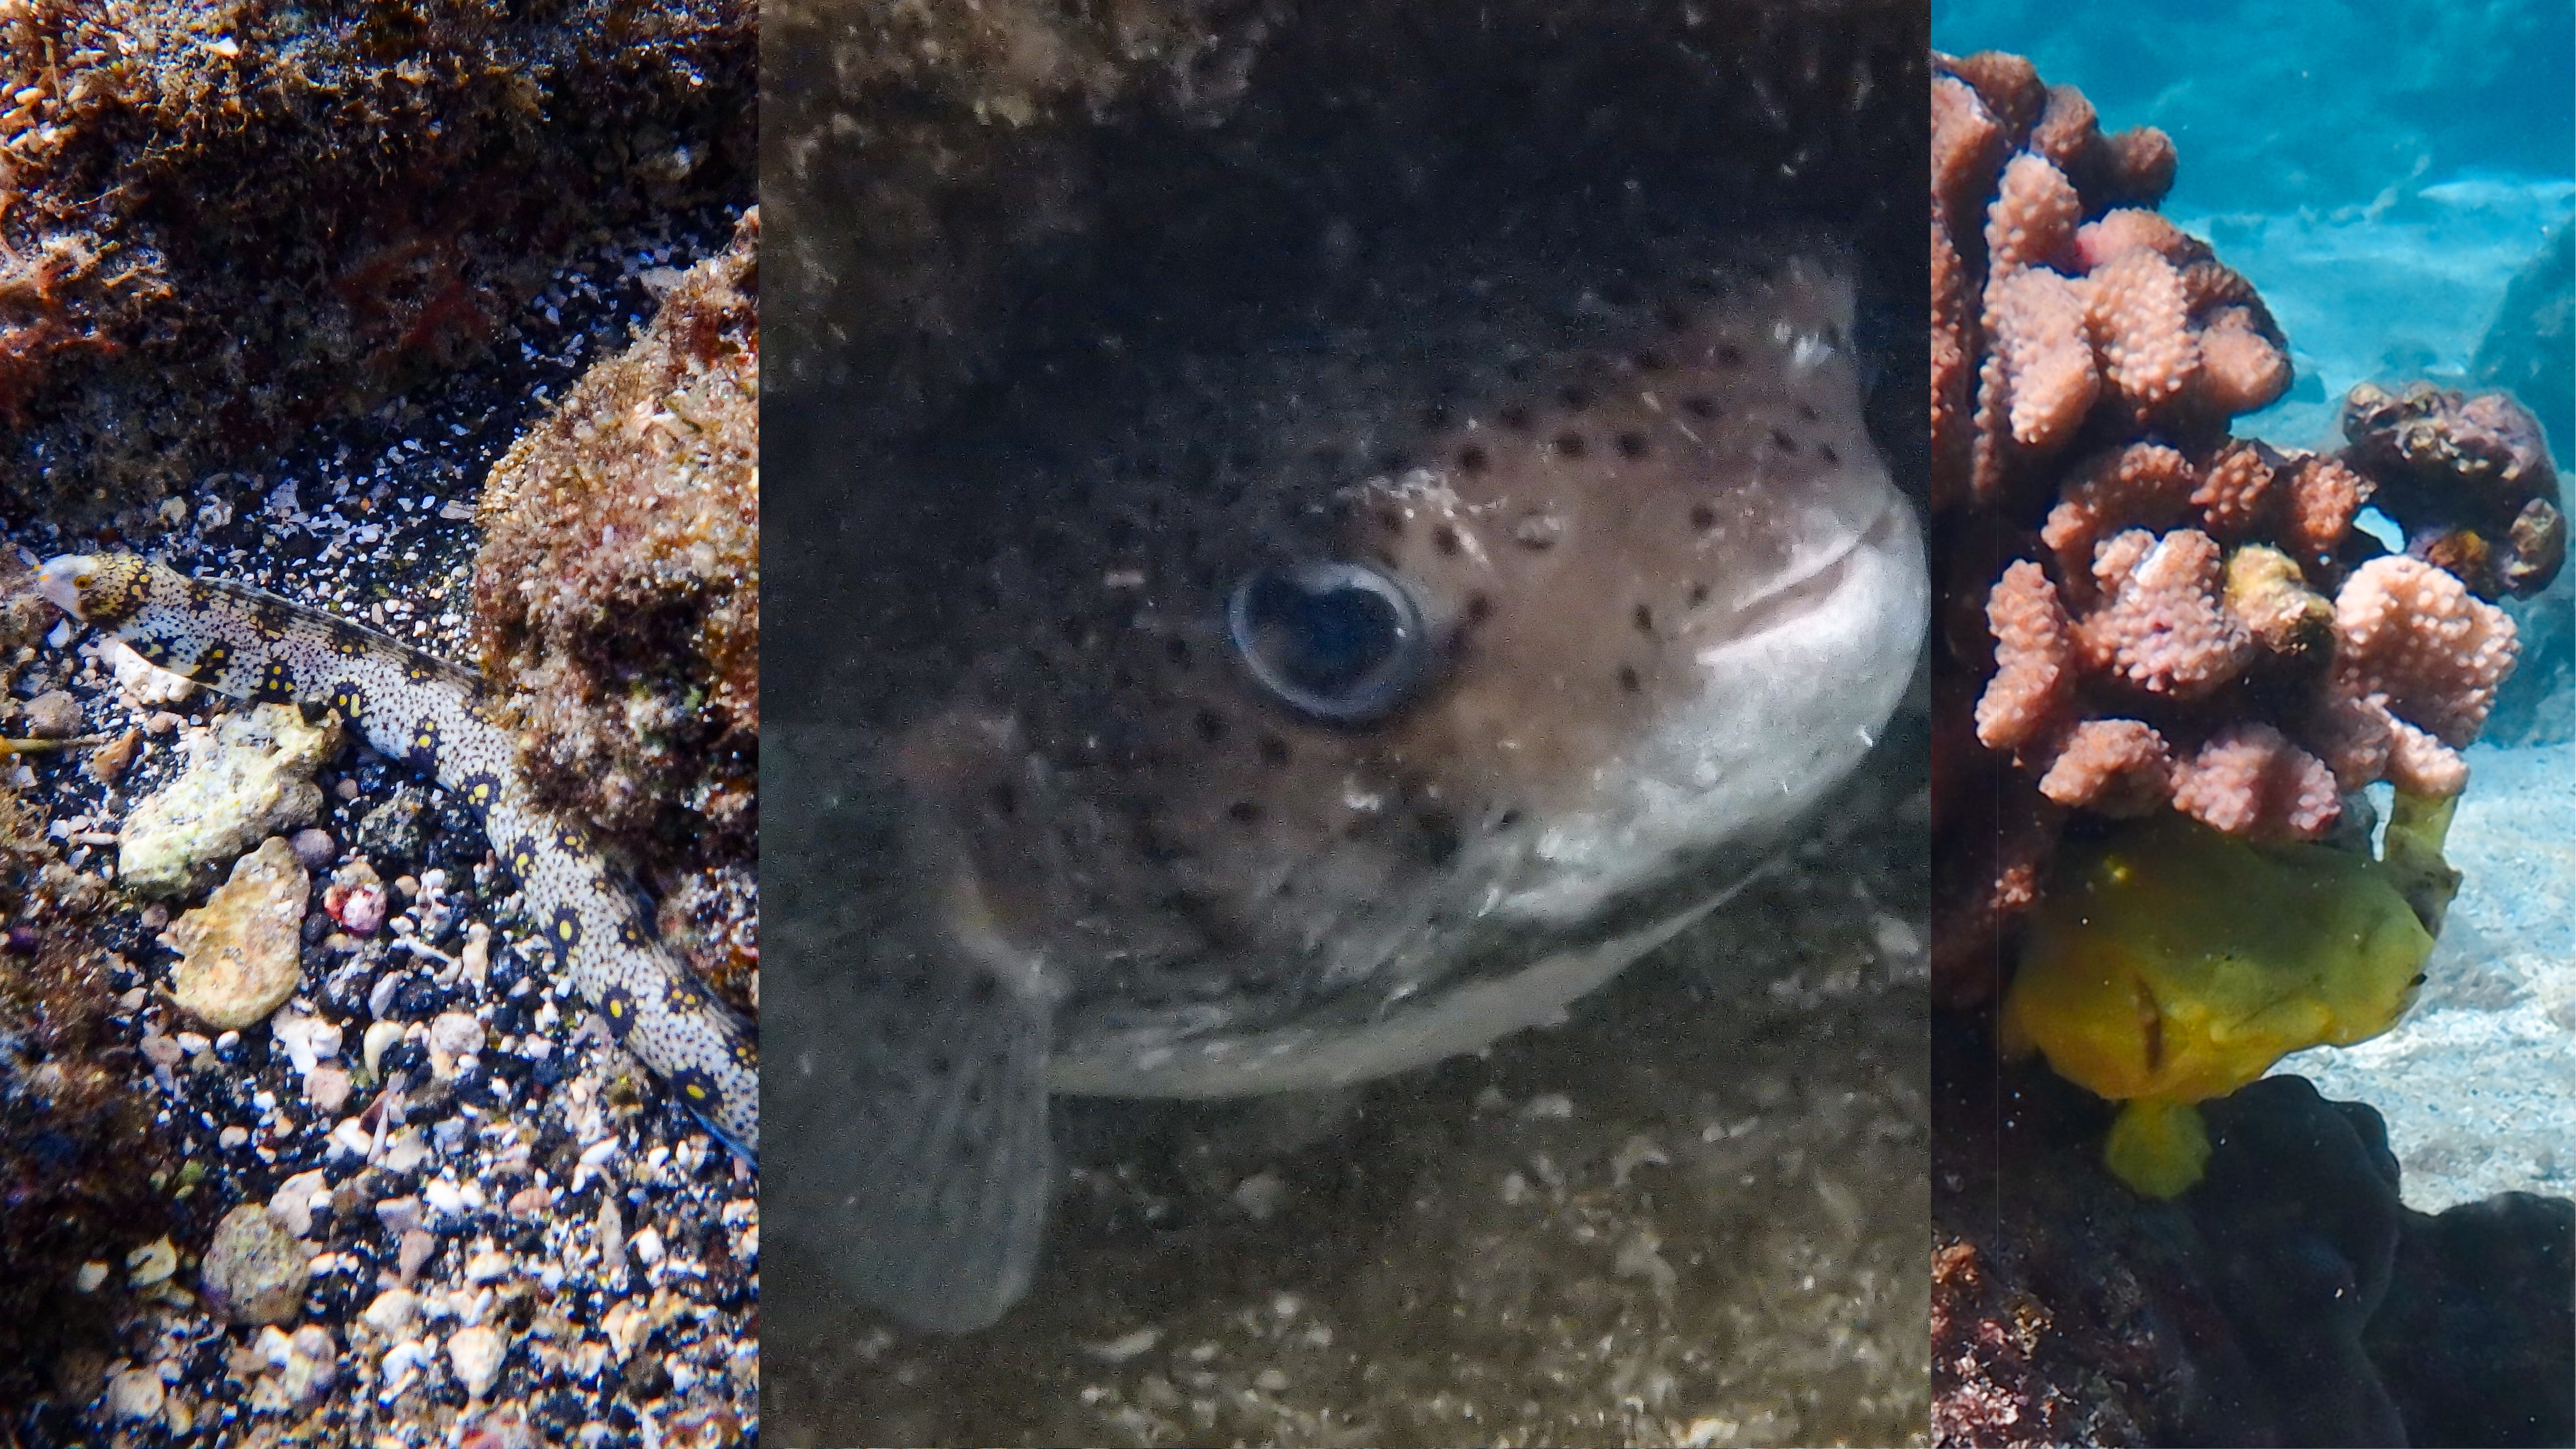
\includegraphics{fish_collage.jpg}

}

\caption{Various fish found in Hawaiʻi. Elke Windschitl 2018.}

\end{figure}

\hypertarget{data}{%
\subsection{Data}\label{data}}

For my analyses I use the IUCN Red List data accessed via the
\href{https://apiv3.iucnredlist.org/}{IUCN Red List API} {[}1{]} and
package rredlist {[}4{]}. Consistent with Munstermann et al., living
species listed as `Vulnerable', `Endangered', or `Critically Endangered'
were categorized as `Threatened'. Living species listed as `Least
Concern' and `Near Threatened' were categorized as `Nonthreatened'
{[}3{]}. Extinct species were not evaluated in this analysis. The IUCN
Red List data are limited in that many marine species have not been
listed yet or have been identified as too data deficient to be
evaluated. The lack of data on elusive fish may introduce bias into the
model.

Fish ecological data were accessed from
\href{https://fishbase.net.br/search.php}{FishBase} {[}5{]} via package
rfishbase {[}6{]}. Different species in the FishBase data were
originally described by different people, possibly leading to errors or
biases. Measurement errors in length may be present, as there are
various common ways to measure the length of a fish. The species
recorded in FishBase may be biased towards fish with commercial value.
Data were wrangled in R and formatted in a tidy data table (Table 1.)

\begin{Shaded}
\begin{Highlighting}[]
\FunctionTok{tab\_df}\NormalTok{(tidy\_fish\_data[}\DecValTok{1}\SpecialCharTok{:}\DecValTok{5}\NormalTok{,],}
       \AttributeTok{title =} \StringTok{"Tbl 1. Hawaii Fish Data"}\NormalTok{,}
       \AttributeTok{col.header =} \FunctionTok{c}\NormalTok{(}\StringTok{"Genus species"}\NormalTok{, }\StringTok{"Length (cm)"}\NormalTok{, }\StringTok{"IUCN Category"}\NormalTok{, }
                          \StringTok{"Common Name"}\NormalTok{, }\StringTok{"Reef Association"}\NormalTok{, }\StringTok{"Endemic"}\NormalTok{,}
                          \StringTok{"Threatened"}\NormalTok{, }\StringTok{"Threatened Binary"}\NormalTok{))}
\end{Highlighting}
\end{Shaded}

\begin{longtable}[]{@{}llllllll@{}}
\caption{Tbl 1. Hawaii Fish Data}\tabularnewline
\toprule()
Genus species & Length (cm) & IUCN Category & Common Name & Reef
Association & Endemic & Threatened & Threatened Binary \\
\midrule()
\endfirsthead
\toprule()
Genus species & Length (cm) & IUCN Category & Common Name & Reef
Association & Endemic & Threatened & Threatened Binary \\
\midrule()
\endhead
Oreochromis mossambicus & 39.00 & VU & Mozambique Tilapia & no & no &
yes & 1 \\
Coryphaena hippurus & 210.00 & LC & Common Dolphinfish & yes & no & no &
0 \\
Coryphaena equiselis & 145.70 & LC & Pompano Dolphinfish & no & no & no
& 0 \\
Alectis indica & 165.00 & LC & Indian Threadfish & yes & no & no & 0 \\
Argyropelecus affinis & 8.40 & LC & Pacific Hatchet Fish & no & no & no
& 0 \\
\bottomrule()
\end{longtable}

\hypertarget{methods}{%
\subsection{Methods}\label{methods}}

Here I run a logistic regression with a categorical binary response
variable of `Threatened' or `Nonthreatened' on species length, coral
reef association, and endemism.

I included length in the model because previous research show that
species of extreme sizes have higher risk of extinction. Ripple et
al.~``found that the probability of being threatened was positively and
significantly related to body mass for birds, cartilaginous fishes, and
mammals'' {[}7{]}. While body mass is not the same as length, the
FishBase data set had few weight entries and many length entries, and
sample size was already limited. Several mass coral bleaching events
have occurred in Hawaiʻi in recent decades causing ecosystem disruption
{[}8{]}. Here I consider if reef-associated fish are more likely to be
threatened than fish that are not reef-associated. Last, endemic species
-- species that are native to a region and occur only in that region --
are known to be at high risk of extinction.

\hypertarget{results-discussion}{%
\subsection{Results \& Discussion}\label{results-discussion}}

\hypertarget{data-exploration}{%
\paragraph{Data exploration:}\label{data-exploration}}

\hypertarget{iucn-red-list-threatened-status}{%
\subparagraph{1. IUCN Red List Threatened
Status}\label{iucn-red-list-threatened-status}}

\begin{Shaded}
\begin{Highlighting}[]
\NormalTok{threat\_tab }\OtherTok{\textless{}{-}} \FunctionTok{table}\NormalTok{(tidy\_fish\_data}\SpecialCharTok{$}\NormalTok{is\_threatened)}
\FunctionTok{tab\_df}\NormalTok{(threat\_tab,}
       \AttributeTok{title  =} \StringTok{"Tbl 2. Counts of threatened species in the data frame"}\NormalTok{,}
       \AttributeTok{col.header =} \StringTok{"Nonthreatened"}\NormalTok{, }\StringTok{"Threatened"}\NormalTok{)}
\end{Highlighting}
\end{Shaded}

\begin{longtable}[]{@{}ll@{}}
\caption{Tbl 2. Counts of threatened species in the data
frame}\tabularnewline
\toprule()
no & yes \\
\midrule()
\endfirsthead
\toprule()
no & yes \\
\midrule()
\endhead
880 & 34 \\
\bottomrule()
\end{longtable}

\hypertarget{fish-length}{%
\subparagraph{2. Fish Length}\label{fish-length}}

\begin{Shaded}
\begin{Highlighting}[]
\FunctionTok{ggplot}\NormalTok{(tidy\_fish\_data, }\FunctionTok{aes}\NormalTok{(}\AttributeTok{x =}\NormalTok{ length\_cm)) }\SpecialCharTok{+}
  \FunctionTok{geom\_histogram}\NormalTok{(}\AttributeTok{fill =} \StringTok{"\#38b6ba"}\NormalTok{, }\AttributeTok{bins =} \DecValTok{60}\NormalTok{) }\SpecialCharTok{+}
  \FunctionTok{theme\_minimal}\NormalTok{() }\SpecialCharTok{+}
  \FunctionTok{labs}\NormalTok{(}\AttributeTok{title =} \StringTok{"Fig 1. Histogram of species length"}\NormalTok{) }\SpecialCharTok{+}
  \FunctionTok{theme}\NormalTok{(}\AttributeTok{panel.background =} \FunctionTok{element\_rect}\NormalTok{(}\AttributeTok{fill =} \StringTok{"\#f7f2e6"}\NormalTok{),}
        \AttributeTok{plot.background =} \FunctionTok{element\_rect}\NormalTok{(}\AttributeTok{fill =} \StringTok{"\#f7f2e6"}\NormalTok{),}
        \AttributeTok{panel.grid.minor =} \FunctionTok{element\_blank}\NormalTok{(),}
        \AttributeTok{panel.grid.major =} \FunctionTok{element\_line}\NormalTok{(}\AttributeTok{colour =} \StringTok{\textquotesingle{}\#c9c9c9\textquotesingle{}}\NormalTok{),}
        \AttributeTok{panel.border =} \FunctionTok{element\_rect}\NormalTok{(}\AttributeTok{colour =} \StringTok{"black"}\NormalTok{, }\AttributeTok{fill=}\ConstantTok{NA}\NormalTok{, }\AttributeTok{size=}\DecValTok{1}\NormalTok{)) }\SpecialCharTok{+}
  \FunctionTok{xlab}\NormalTok{(}\StringTok{"Length (cm)"}\NormalTok{) }\SpecialCharTok{+}
  \FunctionTok{ylab}\NormalTok{(}\StringTok{"Count"}\NormalTok{)}
\end{Highlighting}
\end{Shaded}

\begin{figure}[H]

{\centering \includegraphics{index_files/figure-pdf/unnamed-chunk-5-1.pdf}

}

\end{figure}

\hypertarget{reef-association}{%
\subparagraph{3. Reef-Association}\label{reef-association}}

\begin{Shaded}
\begin{Highlighting}[]
\NormalTok{reef\_tab }\OtherTok{\textless{}{-}} \FunctionTok{table}\NormalTok{(tidy\_fish\_data}\SpecialCharTok{$}\NormalTok{reef\_associated)}
\FunctionTok{tab\_df}\NormalTok{(reef\_tab,}
       \AttributeTok{title =} \StringTok{"Tbl 3. Counts of reef{-}associated species in the data frame"}\NormalTok{)}
\end{Highlighting}
\end{Shaded}

\begin{longtable}[]{@{}ll@{}}
\caption{Tbl 3. Counts of reef-associated species in the data
frame}\tabularnewline
\toprule()
no & yes \\
\midrule()
\endfirsthead
\toprule()
no & yes \\
\midrule()
\endhead
353 & 312 \\
\bottomrule()
\end{longtable}

\hypertarget{endemism}{%
\subparagraph{4. Endemism}\label{endemism}}

\begin{Shaded}
\begin{Highlighting}[]
\NormalTok{end\_tab }\OtherTok{\textless{}{-}} \FunctionTok{table}\NormalTok{(tidy\_fish\_data}\SpecialCharTok{$}\NormalTok{is\_endemic)}
\FunctionTok{tab\_df}\NormalTok{(end\_tab,}
       \AttributeTok{title =} \StringTok{"Tbl 4. Counts of endemic species in the data frame"}\NormalTok{)}
\end{Highlighting}
\end{Shaded}

\begin{longtable}[]{@{}ll@{}}
\caption{Tbl 4. Counts of endemic species in the data
frame}\tabularnewline
\toprule()
no & yes \\
\midrule()
\endfirsthead
\toprule()
no & yes \\
\midrule()
\endhead
895 & 19 \\
\bottomrule()
\end{longtable}

After aligning the FishBase data with the IUCN Red List data, the data
are disproportionate in both the threat level (Table 2) and endemism
(Table 4). Fish length is skewed right (Figure 1), and reef-association
is well balanced (Table 3).

\hypertarget{analysis}{%
\paragraph{Analysis:}\label{analysis}}

\hypertarget{length-operatornamelogitplog-leftfracp1-prightbeta_0beta_1-length-varepsilon}{%
\subparagraph{\texorpdfstring{\textbf{Length}
\[\operatorname{logit}(p)=\log \left(\frac{p}{1-p}\right)=\beta_0+\beta_1  (Length)  +\varepsilon \]}{Length \textbackslash operatorname\{logit\}(p)=\textbackslash log \textbackslash left(\textbackslash frac\{p\}\{1-p\}\textbackslash right)=\textbackslash beta\_0+\textbackslash beta\_1  (Length)  +\textbackslash varepsilon }}\label{length-operatornamelogitplog-leftfracp1-prightbeta_0beta_1-length-varepsilon}}

\begin{Shaded}
\begin{Highlighting}[]
\NormalTok{rm\_len\_na }\OtherTok{\textless{}{-}}\NormalTok{ tidy\_fish\_data }\SpecialCharTok{\%\textgreater{}\%} 
  \FunctionTok{filter}\NormalTok{(}\SpecialCharTok{!}\NormalTok{length\_cm }\SpecialCharTok{==} \StringTok{"NA"}\NormalTok{) }\CommentTok{\# Remove NA length values}
\CommentTok{\# Plot threat prob. vs. length}
\NormalTok{gg\_len }\OtherTok{\textless{}{-}} \FunctionTok{ggplot}\NormalTok{(}\AttributeTok{data =}\NormalTok{ rm\_len\_na, }\FunctionTok{aes}\NormalTok{(}\AttributeTok{x =}\NormalTok{ length\_cm, }
                             \AttributeTok{y =}\NormalTok{ is\_of\_concern)) }\SpecialCharTok{+}
  \FunctionTok{geom\_jitter}\NormalTok{(}\AttributeTok{width =} \DecValTok{0}\NormalTok{, }\AttributeTok{height =} \FloatTok{0.05}\NormalTok{, }
              \AttributeTok{alpha =} \FloatTok{0.8}\NormalTok{, }\AttributeTok{col =} \StringTok{"\#38b6ba"}\NormalTok{) }\SpecialCharTok{+}
  \FunctionTok{theme\_minimal}\NormalTok{() }\SpecialCharTok{+}
  \FunctionTok{labs}\NormalTok{(}\AttributeTok{x =} \StringTok{"Species length (cm)"}\NormalTok{, }
       \AttributeTok{y =} \StringTok{"Listed as threatened"}\NormalTok{, }
       \AttributeTok{title =} \StringTok{"Fig 2. Probability of being threatened by species length"}\NormalTok{) }\SpecialCharTok{+}
  \FunctionTok{theme}\NormalTok{(}\AttributeTok{panel.background =} \FunctionTok{element\_rect}\NormalTok{(}\AttributeTok{fill =} \StringTok{"\#f7f2e6"}\NormalTok{),}
        \AttributeTok{plot.background =} \FunctionTok{element\_rect}\NormalTok{(}\AttributeTok{fill =} \StringTok{"\#f7f2e6"}\NormalTok{),}
        \AttributeTok{panel.grid.minor =} \FunctionTok{element\_blank}\NormalTok{(),}
        \AttributeTok{panel.grid.major =} \FunctionTok{element\_line}\NormalTok{(}\AttributeTok{colour =} \StringTok{\textquotesingle{}\#c9c9c9\textquotesingle{}}\NormalTok{),}
        \AttributeTok{panel.border =} \FunctionTok{element\_rect}\NormalTok{(}\AttributeTok{colour =} \StringTok{"black"}\NormalTok{, }\AttributeTok{fill=}\ConstantTok{NA}\NormalTok{, }\AttributeTok{size=}\DecValTok{1}\NormalTok{))}
\NormalTok{gg\_len }\SpecialCharTok{+} \FunctionTok{geom\_smooth}\NormalTok{(}\AttributeTok{method =} \StringTok{"glm"}\NormalTok{, }
              \AttributeTok{se =} \ConstantTok{FALSE}\NormalTok{, }\AttributeTok{color =} \StringTok{"\#545454"}\NormalTok{, }
              \AttributeTok{method.args =} \FunctionTok{list}\NormalTok{(}\AttributeTok{family =} \StringTok{"binomial"}\NormalTok{))}
\end{Highlighting}
\end{Shaded}

\begin{figure}[H]

{\centering \includegraphics{index_files/figure-pdf/unnamed-chunk-8-1.pdf}

}

\end{figure}

\begin{Shaded}
\begin{Highlighting}[]
\CommentTok{\# Log regression length}
\NormalTok{mod\_length }\OtherTok{\textless{}{-}} \FunctionTok{glm}\NormalTok{(is\_of\_concern }\SpecialCharTok{\textasciitilde{}}\NormalTok{ length\_cm, }
                  \AttributeTok{data =}\NormalTok{ rm\_len\_na, }
                  \AttributeTok{family =} \StringTok{"binomial"}\NormalTok{)}
\CommentTok{\# Model output table format}
\FunctionTok{tab\_model}\NormalTok{(mod\_length,}
          \AttributeTok{transform =} \ConstantTok{NULL}\NormalTok{,}
          \AttributeTok{pred.labels =} \FunctionTok{c}\NormalTok{(}\StringTok{"Intercept"}\NormalTok{, }\StringTok{"Length (cm)"}\NormalTok{),}
          \AttributeTok{dv.labels =} \FunctionTok{c}\NormalTok{(}\StringTok{"log Threat Pobability"}\NormalTok{),}
          \AttributeTok{show.p =} \ConstantTok{TRUE}\NormalTok{,}
          \AttributeTok{p.style =} \FunctionTok{c}\NormalTok{(}\StringTok{"numeric\_stars"}\NormalTok{),}
          \AttributeTok{p.threshold =} \FunctionTok{c}\NormalTok{(}\FloatTok{0.10}\NormalTok{, }\FloatTok{0.05}\NormalTok{, }\FloatTok{0.01}\NormalTok{),}
          \AttributeTok{string.p =} \StringTok{"P{-}value"}\NormalTok{,}
          \AttributeTok{show.r2 =} \ConstantTok{FALSE}\NormalTok{,}
          \AttributeTok{title =} \StringTok{"Tbl 5. Logisitc Regression Model Results for Length"}\NormalTok{,}
          \AttributeTok{digits =} \DecValTok{3}\NormalTok{)}
\end{Highlighting}
\end{Shaded}

\begin{longtable}[]{@{}cccc@{}}
\caption{Tbl 5. Logisitc Regression Model Results for
Length}\tabularnewline
\toprule()
~ & \multicolumn{3}{c}{log Threat Pobability} \\
\midrule()
\endfirsthead
\toprule()
~ & \multicolumn{3}{c}{log Threat Pobability} \\
\midrule()
\endhead
Predictors & Log-Odds & CI & P-value \\
Intercept & -4.505 \textsuperscript{***} & -5.149~--~-3.958 &
\textbf{\textless0.001} \\
Length (cm) & 0.011 \textsuperscript{***} & 0.008~--~0.014 &
\textbf{\textless0.001} \\
Observations & \multicolumn{3}{l}{874} \\
\multicolumn{4}{r}{* p\textless0.1~~~** p\textless0.05~~~***
p\textless0.01} \\
\bottomrule()
\end{longtable}

\begin{Shaded}
\begin{Highlighting}[]
\CommentTok{\# Remove large values to evaluate robustness}
\NormalTok{rm\_outliers }\OtherTok{\textless{}{-}}\NormalTok{ rm\_len\_na }\SpecialCharTok{\%\textgreater{}\%} 
  \FunctionTok{filter}\NormalTok{(length\_cm }\SpecialCharTok{\textless{}=} \DecValTok{1000}\NormalTok{)}
\NormalTok{gg\_rm\_out }\OtherTok{\textless{}{-}} \FunctionTok{ggplot}\NormalTok{(}\AttributeTok{data =}\NormalTok{ rm\_outliers, }\FunctionTok{aes}\NormalTok{(}\AttributeTok{x =}\NormalTok{ length\_cm, }
                                            \AttributeTok{y =}\NormalTok{ is\_of\_concern)) }\SpecialCharTok{+}
  \FunctionTok{geom\_jitter}\NormalTok{(}\AttributeTok{width =} \DecValTok{0}\NormalTok{, }\AttributeTok{height =} \FloatTok{0.05}\NormalTok{, }
              \AttributeTok{alpha =} \FloatTok{0.8}\NormalTok{, }\AttributeTok{col =} \StringTok{"\#38b6ba"}\NormalTok{) }\SpecialCharTok{+}
  \FunctionTok{labs}\NormalTok{(}\AttributeTok{x =} \StringTok{"Species length (cm)"}\NormalTok{, }\AttributeTok{y =} \StringTok{"Listed as threatened"}\NormalTok{, }\AttributeTok{title =} \StringTok{"Fig 3. Probability of being threatened by species length }\SpecialCharTok{\textbackslash{}n}\StringTok{ (excluding outliers)"}\NormalTok{) }\SpecialCharTok{+}
  \FunctionTok{theme\_minimal}\NormalTok{() }\SpecialCharTok{+}
  \FunctionTok{theme}\NormalTok{(}\AttributeTok{panel.background =} \FunctionTok{element\_rect}\NormalTok{(}\AttributeTok{fill =} \StringTok{"\#f7f2e6"}\NormalTok{),}
        \AttributeTok{plot.background =} \FunctionTok{element\_rect}\NormalTok{(}\AttributeTok{fill =} \StringTok{"\#f7f2e6"}\NormalTok{),}
        \AttributeTok{panel.grid.minor =} \FunctionTok{element\_blank}\NormalTok{(),}
        \AttributeTok{panel.grid.major =} \FunctionTok{element\_line}\NormalTok{(}\AttributeTok{colour =} \StringTok{\textquotesingle{}\#c9c9c9\textquotesingle{}}\NormalTok{),}
        \AttributeTok{panel.border =} \FunctionTok{element\_rect}\NormalTok{(}\AttributeTok{colour =} \StringTok{"black"}\NormalTok{, }\AttributeTok{fill=}\ConstantTok{NA}\NormalTok{, }\AttributeTok{size=}\DecValTok{1}\NormalTok{))}
\NormalTok{len\_rm\_out\_plot }\OtherTok{\textless{}{-}}\NormalTok{ gg\_rm\_out }\SpecialCharTok{+}
  \FunctionTok{geom\_smooth}\NormalTok{(}\AttributeTok{method =} \StringTok{"glm"}\NormalTok{, }
              \AttributeTok{se =} \ConstantTok{FALSE}\NormalTok{, }\AttributeTok{color =} \StringTok{"\#545454"}\NormalTok{, }
              \AttributeTok{method.args =} \FunctionTok{list}\NormalTok{(}\AttributeTok{family =} \StringTok{"binomial"}\NormalTok{))}
\NormalTok{len\_rm\_out\_plot}
\end{Highlighting}
\end{Shaded}

\begin{figure}[H]

{\centering \includegraphics{index_files/figure-pdf/unnamed-chunk-8-2.pdf}

}

\end{figure}

\begin{Shaded}
\begin{Highlighting}[]
\CommentTok{\# Log regression length removed outliers}
\NormalTok{mod\_rm\_out }\OtherTok{\textless{}{-}} \FunctionTok{glm}\NormalTok{(is\_of\_concern }\SpecialCharTok{\textasciitilde{}}\NormalTok{ length\_cm, }
                  \AttributeTok{data =}\NormalTok{ rm\_outliers, }
                  \AttributeTok{family =} \StringTok{"binomial"}\NormalTok{)}
\CommentTok{\# Model output table format}
\FunctionTok{tab\_model}\NormalTok{(mod\_rm\_out,}
          \AttributeTok{transform =} \ConstantTok{NULL}\NormalTok{,}
          \AttributeTok{pred.labels =} \FunctionTok{c}\NormalTok{(}\StringTok{"Intercept"}\NormalTok{, }\StringTok{"Length (cm)"}\NormalTok{),}
          \AttributeTok{dv.labels =} \FunctionTok{c}\NormalTok{(}\StringTok{"log Threat Pobability"}\NormalTok{),}
          \AttributeTok{show.p =} \ConstantTok{TRUE}\NormalTok{,}
          \AttributeTok{p.style =} \FunctionTok{c}\NormalTok{(}\StringTok{"numeric\_stars"}\NormalTok{),}
          \AttributeTok{p.threshold =} \FunctionTok{c}\NormalTok{(}\FloatTok{0.10}\NormalTok{, }\FloatTok{0.05}\NormalTok{, }\FloatTok{0.01}\NormalTok{),}
          \AttributeTok{string.p =} \StringTok{"P{-}value"}\NormalTok{,}
          \AttributeTok{show.r2 =} \ConstantTok{FALSE}\NormalTok{,}
          \AttributeTok{title =} \StringTok{"Tbl 6. Logisitc Regression Model Results for Length with Outliers Removed"}\NormalTok{,}
          \AttributeTok{digits =} \DecValTok{3}\NormalTok{)}
\end{Highlighting}
\end{Shaded}

\begin{longtable}[]{@{}cccc@{}}
\caption{Tbl 6. Logisitc Regression Model Results for Length with
Outliers Removed}\tabularnewline
\toprule()
~ & \multicolumn{3}{c}{log Threat Pobability} \\
\midrule()
\endfirsthead
\toprule()
~ & \multicolumn{3}{c}{log Threat Pobability} \\
\midrule()
\endhead
Predictors & Log-Odds & CI & P-value \\
Intercept & -4.505 \textsuperscript{***} & -5.149~--~-3.958 &
\textbf{\textless0.001} \\
Length (cm) & 0.011 \textsuperscript{***} & 0.008~--~0.014 &
\textbf{\textless0.001} \\
Observations & \multicolumn{3}{l}{872} \\
\multicolumn{4}{r}{* p\textless0.1~~~** p\textless0.05~~~***
p\textless0.01} \\
\bottomrule()
\end{longtable}

\begin{Shaded}
\begin{Highlighting}[]
\CommentTok{\# Compute fitted probabilities}
\NormalTok{length\_plus }\OtherTok{\textless{}{-}}\NormalTok{ mod\_length }\SpecialCharTok{\%\textgreater{}\%}
  \FunctionTok{augment}\NormalTok{(}\AttributeTok{type.predict =} \StringTok{"response"}\NormalTok{) }\SpecialCharTok{\%\textgreater{}\%}
  \FunctionTok{mutate}\NormalTok{(}\AttributeTok{y\_hat =}\NormalTok{ .fitted)}
\CommentTok{\# Compute odds scale}
\NormalTok{length\_plus }\OtherTok{\textless{}{-}}\NormalTok{ length\_plus }\SpecialCharTok{\%\textgreater{}\%} 
  \FunctionTok{mutate}\NormalTok{(}\AttributeTok{odds\_hat =}\NormalTok{ y\_hat }\SpecialCharTok{/}\NormalTok{ (}\DecValTok{1} \SpecialCharTok{{-}}\NormalTok{ y\_hat)) }\SpecialCharTok{\%\textgreater{}\%} 
  \FunctionTok{filter}\NormalTok{(length\_cm }\SpecialCharTok{\textless{}=} \DecValTok{1000}\NormalTok{) }\CommentTok{\# remove outliers for graphing}
\CommentTok{\# Graph odds scale}
\NormalTok{len\_odds\_plot }\OtherTok{\textless{}{-}} \FunctionTok{ggplot}\NormalTok{(length\_plus, }\FunctionTok{aes}\NormalTok{(}\AttributeTok{x =}\NormalTok{ length\_cm, }
                                         \AttributeTok{y =}\NormalTok{ odds\_hat)) }\SpecialCharTok{+}
  \FunctionTok{geom\_point}\NormalTok{() }\SpecialCharTok{+} 
  \FunctionTok{geom\_line}\NormalTok{() }\SpecialCharTok{+} 
  \FunctionTok{scale\_y\_continuous}\NormalTok{(}\StringTok{"Odds of being threatened"}\NormalTok{) }\SpecialCharTok{+}
  \FunctionTok{labs}\NormalTok{(}\AttributeTok{x =} \StringTok{"Species length (cm)"}\NormalTok{, }
       \AttributeTok{title =} \StringTok{"Fig 4. Odds of being threatened by species length"}\NormalTok{) }\SpecialCharTok{+}
  \FunctionTok{theme\_minimal}\NormalTok{() }\SpecialCharTok{+}
  \FunctionTok{theme}\NormalTok{(}\AttributeTok{panel.background =} \FunctionTok{element\_rect}\NormalTok{(}\AttributeTok{fill =} \StringTok{"\#f7f2e6"}\NormalTok{),}
        \AttributeTok{plot.background =} \FunctionTok{element\_rect}\NormalTok{(}\AttributeTok{fill =} \StringTok{"\#f7f2e6"}\NormalTok{),}
        \AttributeTok{panel.grid.minor =} \FunctionTok{element\_blank}\NormalTok{(),}
        \AttributeTok{panel.grid.major =} \FunctionTok{element\_line}\NormalTok{(}\AttributeTok{colour =} \StringTok{\textquotesingle{}\#c9c9c9\textquotesingle{}}\NormalTok{),}
        \AttributeTok{panel.border =} \FunctionTok{element\_rect}\NormalTok{(}\AttributeTok{colour =} \StringTok{"black"}\NormalTok{, }\AttributeTok{fill=}\ConstantTok{NA}\NormalTok{, }\AttributeTok{size=}\DecValTok{1}\NormalTok{))}
\NormalTok{len\_odds\_plot}
\end{Highlighting}
\end{Shaded}

\begin{figure}[H]

{\centering \includegraphics{index_files/figure-pdf/unnamed-chunk-9-1.pdf}

}

\end{figure}

Here we see that longer fish are associated with higher probability of
being threatened (Table 5, p-value = \textless0.001), but two outliers
may be driving this significance (Figure 2). However, when the outliers
are removed, we still see a significant positive correlation between
fish length and probability of threat (Table 6, p-value =
\textless0.001) with the 50\% probability mark remaining just over 400
cm (Figure 3). When we compute the odds ratio, we see that there is an
exponential relationship between the length and the odds of a species
being threatened. Odds of being threatened increase more at large
lengths (Figure 4).

Confusion Matrix:

\begin{Shaded}
\begin{Highlighting}[]
\NormalTok{length\_plus }\OtherTok{\textless{}{-}} \FunctionTok{augment}\NormalTok{(mod\_length, }\AttributeTok{type.predict =} \StringTok{"response"}\NormalTok{) }\SpecialCharTok{\%\textgreater{}\%}
  \FunctionTok{mutate}\NormalTok{(}\AttributeTok{threatened\_hat =} \FunctionTok{round}\NormalTok{(.fitted)) }\SpecialCharTok{\%\textgreater{}\%}
  \FunctionTok{select}\NormalTok{(is\_of\_concern, length\_cm, .fitted, threatened\_hat)}
\NormalTok{l\_con\_matrix }\OtherTok{\textless{}{-}}\NormalTok{ length\_plus }\SpecialCharTok{\%\textgreater{}\%}
  \FunctionTok{select}\NormalTok{(is\_of\_concern, threatened\_hat) }\SpecialCharTok{\%\textgreater{}\%}
  \FunctionTok{table}\NormalTok{()}
\NormalTok{rownames }\OtherTok{\textless{}{-}} \FunctionTok{c}\NormalTok{(}\StringTok{"Actually Nonthreatened"}\NormalTok{, }\StringTok{"Actually Threatend"}\NormalTok{)}
\NormalTok{colnames }\OtherTok{\textless{}{-}} \FunctionTok{c}\NormalTok{(}\StringTok{"Predicted Nonthreatend"}\NormalTok{, }\StringTok{"Predicted Threatened"}\NormalTok{)}
\NormalTok{l\_con\_matrix }\OtherTok{\textless{}{-}} \FunctionTok{as.data.frame}\NormalTok{(}\FunctionTok{matrix}\NormalTok{(}\FunctionTok{c}\NormalTok{(l\_con\_matrix[}\DecValTok{1}\NormalTok{], }
\NormalTok{                                       l\_con\_matrix[}\DecValTok{2}\NormalTok{], }
\NormalTok{                                       l\_con\_matrix[}\DecValTok{3}\NormalTok{], }
\NormalTok{                                       l\_con\_matrix[}\DecValTok{4}\NormalTok{]), }
                                     \AttributeTok{ncol =} \DecValTok{2}\NormalTok{, }
                                     \AttributeTok{nrow =} \DecValTok{2}\NormalTok{),}
                              \AttributeTok{row.names =}\NormalTok{ rownames)}
\FunctionTok{colnames}\NormalTok{(l\_con\_matrix) }\OtherTok{\textless{}{-}}\NormalTok{ colnames}
\FunctionTok{tab\_df}\NormalTok{(l\_con\_matrix,}
       \AttributeTok{title =} \StringTok{"Tbl 7. Confusion Matrix Displaying Lenght Model Performance"}\NormalTok{,}
       \AttributeTok{show.rownames =} \ConstantTok{TRUE}\NormalTok{)}
\end{Highlighting}
\end{Shaded}

\begin{longtable}[]{@{}lll@{}}
\caption{Tbl 7. Confusion Matrix Displaying Lenght Model
Performance}\tabularnewline
\toprule()
Row & Predicted.Nonthreatend & Predicted.Threatened \\
\midrule()
\endfirsthead
\toprule()
Row & Predicted.Nonthreatend & Predicted.Threatened \\
\midrule()
\endhead
Actually Nonthreatened & 835 & 5 \\
Actually Threatend & 22 & 12 \\
\bottomrule()
\end{longtable}

The accuracy of the model is 97\% with 847 out of 874 predicted
observations being correct (Table 7). However, the model seems to be
more accurate in predicting species that are not actually of concern
(true negative rate = 0.99). Species that are threatened have poorer
prediction rates (true positive rate = 0.38).

\hypertarget{full-model-operatornamelogitplog-leftfracp1-prightbeta_0beta_1-length-beta_2-reef-beta_3-endemic-varepsilon}{%
\subparagraph{\texorpdfstring{\textbf{Full Model}
\[\operatorname{logit}(p)=\log \left(\frac{p}{1-p}\right)=\beta_0+\beta_1  (Length) + \beta_2  (Reef) + \beta_3  (Endemic) +\varepsilon \]}{Full Model \textbackslash operatorname\{logit\}(p)=\textbackslash log \textbackslash left(\textbackslash frac\{p\}\{1-p\}\textbackslash right)=\textbackslash beta\_0+\textbackslash beta\_1  (Length) + \textbackslash beta\_2  (Reef) + \textbackslash beta\_3  (Endemic) +\textbackslash varepsilon }}\label{full-model-operatornamelogitplog-leftfracp1-prightbeta_0beta_1-length-beta_2-reef-beta_3-endemic-varepsilon}}

\begin{Shaded}
\begin{Highlighting}[]
\FunctionTok{tab\_model}\NormalTok{(mod,}
          \AttributeTok{transform =} \ConstantTok{NULL}\NormalTok{,}
          \AttributeTok{pred.labels =} \FunctionTok{c}\NormalTok{(}\StringTok{"Intercept"}\NormalTok{, }\StringTok{"Length (cm)"}\NormalTok{, }
                          \StringTok{"Reef Association"}\NormalTok{, }\StringTok{"Endemic"}\NormalTok{),}
          \AttributeTok{dv.labels =} \FunctionTok{c}\NormalTok{(}\StringTok{"log Threat Pobability"}\NormalTok{),}
          \AttributeTok{p.style =} \FunctionTok{c}\NormalTok{(}\StringTok{"numeric\_stars"}\NormalTok{),}
          \AttributeTok{p.threshold =} \FunctionTok{c}\NormalTok{(}\FloatTok{0.10}\NormalTok{, }\FloatTok{0.05}\NormalTok{, }\FloatTok{0.01}\NormalTok{),}
          \AttributeTok{show.p =} \ConstantTok{TRUE}\NormalTok{,}
          \AttributeTok{string.p =} \StringTok{"P{-}value"}\NormalTok{,}
          \AttributeTok{show.r2 =} \ConstantTok{FALSE}\NormalTok{,}
          \AttributeTok{title =} \StringTok{"Tbl 8. Logisitc Regression Model Results for Length, Reef Association, and Endemism"}\NormalTok{,}
          \AttributeTok{digits =} \DecValTok{3}\NormalTok{)}
\end{Highlighting}
\end{Shaded}

\begin{longtable}[]{@{}cccc@{}}
\caption{Tbl 8. Logisitc Regression Model Results for Length, Reef
Association, and Endemism}\tabularnewline
\toprule()
~ & \multicolumn{3}{c}{log Threat Pobability} \\
\midrule()
\endfirsthead
\toprule()
~ & \multicolumn{3}{c}{log Threat Pobability} \\
\midrule()
\endhead
Predictors & Log-Odds & CI & P-value \\
Intercept & -4.431 \textsuperscript{***} & -5.324~--~-3.694 &
\textbf{\textless0.001} \\
Length (cm) & 0.011 \textsuperscript{***} & 0.008~--~0.014 &
\textbf{\textless0.001} \\
Reef Association & -0.048 \textsuperscript{} & -0.972~--~0.869 &
0.918 \\
Endemic & 1.989 \textsuperscript{*} & -0.972~--~3.798 & 0.071 \\
Observations & \multicolumn{3}{l}{650} \\
\multicolumn{4}{r}{* p\textless0.1~~~** p\textless0.05~~~***
p\textless0.01} \\
\bottomrule()
\end{longtable}

We can see from the output above that length remains significant (Table
8, p-value = \textless0.001) even when additional variables are added,
making length robust. Endemicity is a significant predictor of threat
probability at a significance level of 0.10 (p-value = 0.0707). Coral
reef association is not significantly impacting the model (p-value =
0.9175).

\hypertarget{predicting-probability-solving-for-p}{%
\paragraph{Predicting Probability -- Solving for
p:}\label{predicting-probability-solving-for-p}}

In this model, the smallest fish in the data set -- \emph{Melamphaes
danae} (bigscale) at 2.30 cm -- has a probability of being threatened of
0.012. The largest fish in the data set -- \emph{Rhincodon typus} (whale
shark) at 1700 cm -- has a probability of being threatened of 0.99. Here
I use the model to predict the probabilities of being threatened for
unlisted fish.

\begin{Shaded}
\begin{Highlighting}[]
\NormalTok{tidy\_pred\_rank }\OtherTok{\textless{}{-}}\NormalTok{ tidy\_pred\_rank }\SpecialCharTok{\%\textgreater{}\%} 
  \FunctionTok{select}\NormalTok{(}\StringTok{"genus\_species"}\NormalTok{, }\StringTok{"length\_cm"}\NormalTok{, }\StringTok{"coral\_reefs"}\NormalTok{, }\StringTok{"main\_common\_name"}\NormalTok{, }\StringTok{"reef\_associated"}\NormalTok{, }\StringTok{"endemic"}\NormalTok{, }\StringTok{"y\_hat"}\NormalTok{)}
\FunctionTok{tab\_df}\NormalTok{(tidy\_pred\_rank[}\DecValTok{1}\SpecialCharTok{:}\DecValTok{5}\NormalTok{,],}
       \AttributeTok{title =} \StringTok{"Tbl 9. Top 5 Most Vulnerable Unranked Fish in Hawaii"}\NormalTok{,}
       \AttributeTok{col.header =} \FunctionTok{c}\NormalTok{(}\StringTok{"Genus species"}\NormalTok{, }\StringTok{"Length (cm)"}\NormalTok{, }\StringTok{"Reef Association"}\NormalTok{,}
                          \StringTok{"Common Name"}\NormalTok{, }\StringTok{"Reef Association"}\NormalTok{, }\StringTok{"Endemic"}\NormalTok{,}
                          \StringTok{"Threatened"}\NormalTok{))}
\end{Highlighting}
\end{Shaded}

\begin{longtable}[]{@{}lllllll@{}}
\caption{Tbl 9. Top 5 Most Vulnerable Unranked Fish in
Hawaii}\tabularnewline
\toprule()
Genus species & Length (cm) & Reef Association & Common Name & Reef
Association & Endemic & Threatened \\
\midrule()
\endfirsthead
\toprule()
Genus species & Length (cm) & Reef Association & Common Name & Reef
Association & Endemic & Threatened \\
\midrule()
\endhead
Makaira mazara & 500 & 0 & NA & no & no & 0.74 \\
Istiompax indica & 465 & 1 & Black Marlin & yes & no & 0.65 \\
Echinorhinus cookei & 400 & 0 & Prickly Shark & no & no & 0.49 \\
Epinephelus lanceolatus & 270 & 1 & Giant Grouper & yes & no & 0.18 \\
Assurger anzac & 250 & 0 & NA & no & no & 0.15 \\
\bottomrule()
\end{longtable}

The top five most vulnerable unranked species under this model are
\emph{Makaira mazara} (Indo-Pacific blue marlin), \emph{Istiompax
indica} (black marlin), \emph{Echinorhinus cookei} (prickly shark),
\emph{Epinephelus lanceolatus} (giant grouper), and \emph{Assurger
anzac} (razorback scabbardfish) (Table 9.) \emph{Makaira mazara} and
\emph{Istiompax indica} have probabilities of being threatened over
50\%. I would recommend the IUCN evaluate these two species before
others. However, there are limitations to this analysis and more
research should be done before allocating resources to evaluate these
species.

\hypertarget{limitations-next-steps}{%
\subsection{Limitations \& Next Steps}\label{limitations-next-steps}}

As mentioned above, both the IUCN Red List data and the FishBase data
have potential biases and don't evaluate all species. Additionally, not
all listed species had every piece of information, and missing data were
removed. With missing data removed, the sample became small. It is
possible that endemism plays a bigger role in threat risk than
illustrated here by the model. Points of concern with this model include
disproportionate data in both the threat level and endemism, and high
false negative rates in binary prediction. Future analyses could
investigate other potential explanatory variables such as metrics
measuring fishing pressure, life cycle characteristics, and range.
Future analyses should also incorporate indigenous knowledge as Native
People in Hawaiʻi know fish history around the islands and are
frequently in the water for spearfishing and other recreation.
Additionally, future analyses could expand the area of interest to all
of the tropics.

Reference

{[}1{]} ``IUCN,'' IUCN Red List of Threatened Species. Version 2022-1,
2022. https://www.iucnredlist.org/ (accessed Dec.~02, 2022).

{[}2{]} B. J. Cardinale et al., ``Biodiversity loss and its impact on
humanity,'' Nature, vol.~486, no. 7401, Art. no. 7401, Jun.~2012, doi:
10.1038/nature11148. {[}3{]} M. J. Munstermann et al., ``A global
ecological signal of extinction risk in terrestrial vertebrates,''
Conserv. Biol., vol.~36, no. 3, p.~e13852, 2022, doi:
10.1111/cobi.13852.

{[}4{]} ``IUCN,'' IUCN Red List of Threatened Species. Version 2022-1,
2015. www.iucnredlist.org

{[}5{]} R. Froese and D. Pauly, ``FishBase,'' 2022. www.fishbase.org

{[}6{]} C. Boettiger, D. Temple Lang, and P. Wainwright, ``rfishbase:
exploring, manipulating and visualizing FishBase data from R.,'' J. Fish
Biol., 2012, doi: https://doi.org/10.1111/j.1095-8649.2012.03464.x.

{[}7{]} W. J. Ripple, C. Wolf, T. M. Newsome, M. Hoffmann, A. J.
Wirsing, and D. J. McCauley, ``Extinction risk is most acute for the
world's largest and smallest vertebrates,'' Proc. Natl. Acad. Sci. U. S.
A., vol.~114, no. 40, pp.~10678--10683, Oct.~2017, doi:
10.1073/pnas.1702078114.

{[}8{]} K. D. Bahr, P. L. Jokiel, and K. S. Rodgers, ``The 2014 coral
bleaching and freshwater flood events in Kāneʻohe Bay, Hawaiʻi,'' PeerJ,
vol.~3, p.~e1136, Aug.~2015, doi: 10.7717/peerj.1136.



\end{document}
